\documentclass[12pt]{article}
\usepackage[margin=1in]{geometry}
\usepackage{fancyvrb}
\usepackage{multicol}
\usepackage{hyperref}
\usepackage{amsmath}
\usepackage{amsfonts}

\usepackage[listings]{tcolorbox}

\definecolor{codegreen}{rgb}{0,0.6,0}
\definecolor{codegray}{rgb}{0.5,0.5,0.5}
\definecolor{codepurple}{rgb}{0.58,0,0.82}
\definecolor{backcolour}{rgb}{0.95,0.95,0.92}

\lstdefinestyle{mystyle}{
    language=Python,
    backgroundcolor=\color{backcolour},   
    commentstyle=\color{codegreen},
    keywordstyle=\color{magenta},
    numberstyle=\tiny\color{codegray},
    stringstyle=\color{codepurple},
    basicstyle=\ttfamily\footnotesize,
    breakatwhitespace=false,         
    breaklines=true,                 
    captionpos=b,                    
    keepspaces=true,                 
    numbers=left,                    
    numbersep=5pt,                  
    showspaces=false,                
    showstringspaces=false,
    showtabs=false,                  
    tabsize=2,
    escapechar=|,
    frame=single
}

\lstset{style=mystyle}

\newcommand{\showfig}[2]{
\noindent\includegraphics[width=\textwidth]{#1}
\centerline{#1}
}

\begin{document}
\sloppy
\centerline{\Large CSCI 111, Bonus Lab 3}
\centerline{\large Histogram equalization}


\begin{description}

\item[Individual work:]  All work must be your own.  Do not share
code with anyone other than the instructor and teaching assistants.
This includes looking over shoulders at screens with the code open.
You may discuss ideas, algorithms, approaches, {\em etc.} with
other students but NEVER actual code.

\item[Histogram equalization:]
This is an addition to lab 7, which processed images
using different filters.

A very useful filter for contrast enhancement is
histogram equalization.  As an example, here I am
in an original grayscale and an enhanced contrast
version:

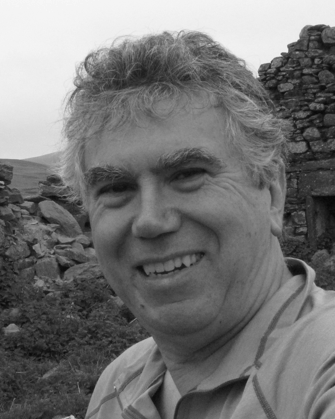
\includegraphics[scale=0.5]{greyscalegeoff}\hfill
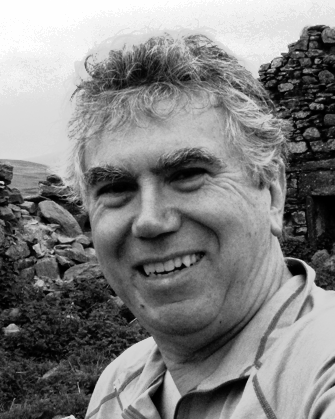
\includegraphics[scale=0.5]{equalizedgeoff}

This is accomplished by creating a histogram of
brightness values.  It will be best if you use
integers for brightness values. You can use 0..255 for the
brightness values if you like, it makes things
simpler.  Each brightness
value (or luminance) is used as a key in a dictionary,
and the number of times it occurse in an image is
counted.

We then find the cumulative histogram for the image,
where each success brightness in the dictionary
stores the {\bf sum} of all previous brightness
entries.

If the total number of brightness entries is \lstinline{n},
(the sum of the values in the histogram, or the 
last value in the cumulative histogram),
then the new brightness of a pixel with
brightness level \lstinline{brightness_level} is
\begin{lstlisting}
   cumulstive_histogram[brightness_level]/n
\end{lstlisting}
This is a number between 0 and 1, so you can
scale it to 255 to get the final image brightness
for the pixel.


\end{description}

\end{document}
